\section{Условие}
{\bfseries Цель работы:} Научиться использовать интерфейсы управления и конфигурирования оборудования $Cisco Systems$ и $Mikrotik$, настраивать ip-адреса устройств, пароли и логины, настраивать конечный пользовательский $NAT$ на $Mikrotik$.

{\bfseries Вариант:} 29.

\begin{figure}[h!]
    \centering
    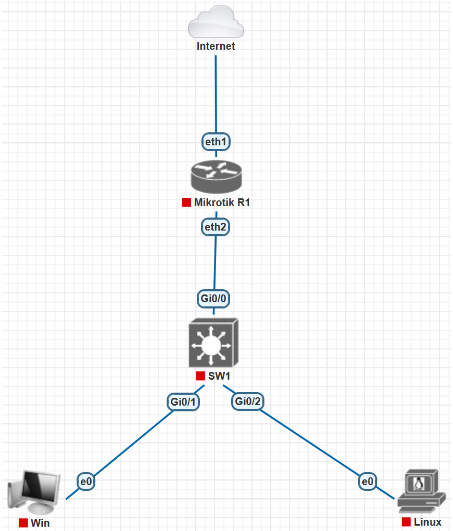
\includegraphics[]{./img/sheme.png}
    \caption{Схема сети}
\end{figure}

{\bfseries Задачи:}
\begin{enumerate}
    \item Настроить имена узлов для коммутатора и маршрутизатора в соответствии с именами, указанными в топологии ($SW1$ и $R1$).
    \item Сменить пароль администратора (пароль доступа к привилегированному режиму $enable$ для $Cisco$) на вариант ЛР для соответствующего устройства.
    \item Создать пользователя $checker$ с максимальным административным уровнем доступа и паролем “PfxtvXtrth!” без кавычек на коммутаторе и маршрутизаторе.
    \item Настроить на маршрутизаторе $R1$ IP-адреса интерфейсов в соответствии с вариантом задания.
    \item Настроить на коммутаторе $SW1$ IP-адрес в соответствии с вариантом задания, адрес DNS-сервера ($192.168.N.1$) и маршрут по умолчанию в управляющем $VLAN$.
    \item Настроить на маршрутизаторе $R1$ встроенный DNS-сервер с передачей запросов на сервер $QuadNine$ ($9.9.9.9$), вкачу адресолючить удаленные запросы.
    \item Настроить на маршрутизаторе $R1$ раздав с помощью $DHCP$ из внутреннего пула, указанного в варианте задания с указанием в качестве маршрута по умолчанию и DNS-сервера внутреннего IP-адреса маршрутизатора $R1$ ($eth2$).
    \item Настроить на маршрутизаторе $R1$ трансляцию сетевых адресов ($NAT$) из адресов внутренней сети в адрес на внешнем интерфейсе маршрутизатора ($eth1$).
    \item Включить на коммутаторе и маршрутизаторе доступ по протоколу $ssh$, выключить web-интерфейсы коммутатора, убедиться, что доступ по $ssh$ работает с хостов в сети для администратора и пользователя $checker$.
    \item Убедиться в работоспособности сети путем проверки разрешения имен в сети Интернет, работоспособности $ping/traceroute$ и открытия веб-сайтов с хостов $Win$ и $Linux$ в топологии в режиме автоматической настройки интерфейсов с помощью $DHCP$.  
\end{enumerate}

{\bfseries Допустимые средства конфигурации:} На хосте Win имеется установленный $WinBox$ для конфигурации $Mikrotik$, его разрешается использовать. Также разрешается использовать консоль маршрутизатора и коммутатора без ограничений. Запрещается использовать web-интерфейс для настройки коммутатора.

\pagebreak